\section{System}
\label{sec:sys}

\begin{figure}[t]
\centering
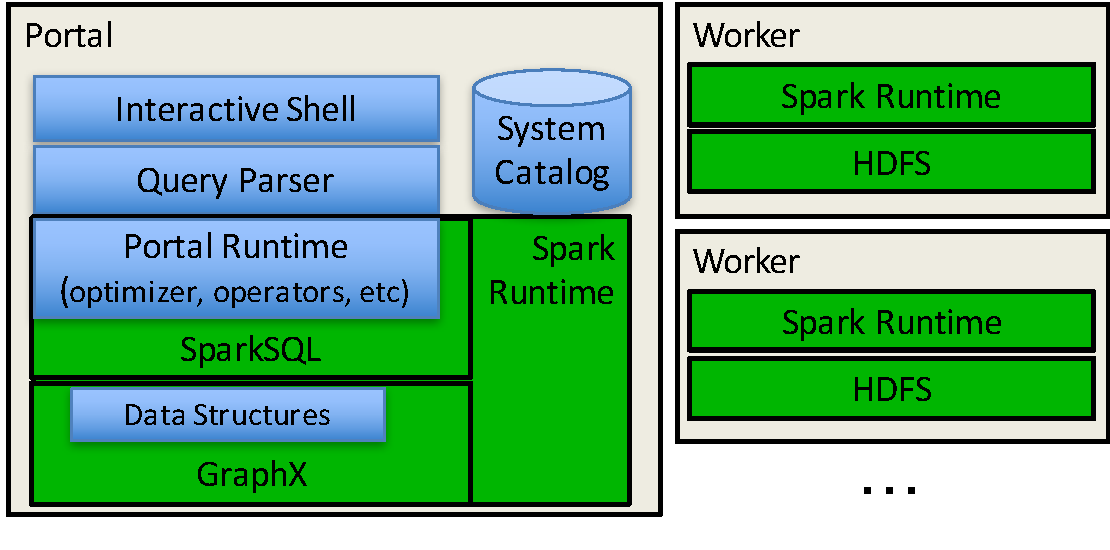
\includegraphics[width=3in]{figs/architecture.pdf}
\vspace{-0.5cm}
\caption{\sys system architecture.}
\vspace{-0.5cm}
\label{fig:arch}
\end{figure}

We developed a prototype system \sys that is implemented on top of
Apache Spark/GraphX~\cite{DBLP:conf/osdi/GonzalezXDCFS14}/Spark
SQL~\cite{Armbrust2015}, as depicted in Figure~\ref{fig:arch}.  Green
boxes indicate built-in components, while blue are those we added for
\sys.  Data is distributed in partitions across the cluster workers,
is read in from the distributed file system (HDFS), and can be viewed
both as a graph and as a pair of RDDs.  All \tg operations are
available through the public API of the \sys library, and may be used
in an Apache Spark application.

{\bf Temporal operators.}  Apache Spark is not a temporal DBMS but
rather an open-source in-memory distributed framework that combines
graph-parallel and data-parallel abstractions.  We reduce our temporal
operators into a sequence of non-temporal relational operators or
their equivalents for Spark RDDs, maintaining point semantics.  While
the TGA is based on relational algebra, multiple transformations are
required for some operations and we use other, more efficient, access
methods where it makes sense.  In some cases, such as temporal window
node creation, access methods based on GraphX graphs provide
significantly more efficient performance.  For analytics, we use the
GraphX Pregel library, but add a batching method to compute overall
time instances together, see~\cite{MoffittTempWeb16} for a detailed
discussion.\eat{ \sys supports PageRank, connected components, and
  shortest paths analytics out of the box, and provides an API for
  adding others.  We are in the process of adding the clustering
  coefficient analytic.}

{\bf Query evaluation.}  \sys query execution follows the traditional
query processing steps: parsing, logical plan generation and
verification, and physical plan generation. \sys re-uses and extends
SparkSQL classes for these steps, including expressions, query tree,
etc, but not the SparkSQL execution engine.  A \ql query is rewritten
into a sequence of \tga operators, and some operators are reordered in
a rule-based manner to improve performance.

Similar to SQL, we apply attribute pruning (column pruning in SQL) and
collapse multiple filters into one.  Slice is always pushed to the
bottom of the tree, except when it appears after temporal window node
creation.  We also add slice to each subtree of the query execution
plan of temporal intersection, based on information about temporal
ranges of \tgs stored in the system catalog.  \eat{E-subgraph is
  pushed through v-subgraph if e-subgraph has no temporal predicate
  because this leads to smaller join size in v-subgraph during
  integrity constraint enforcement.}Unlike selection in SQL, filters
cannot be pushed down through union because of the aggregation
functions.  (See extended discussion on the need for aggregation
functions in set-based operators in~\cite{PortalarXiv2016}).
Attribute-based node creation is always placed before temporal node
creation and temporal union, because it leads to a reduction in
intermediate result size.

We developed several physical representations and partitioning
strategies, selected at the physical plan generation stage.  One
representation mirrors the logical data model and translates \tga
operators into RDD transformations.  Other representations are
graph-based, use the GraphX library, and are more efficient under
certain conditions.  \tgs are read into memory from HDFS and processed
by Spark Workers, with task assignment managed by the runtime.
Details can be found in~\cite{PortalarXiv2016}.

\begin{figure}[t]
\centering
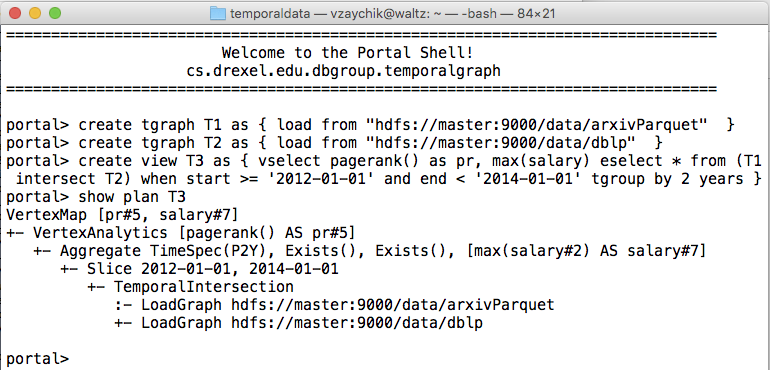
\includegraphics[width=3.4in]{figs/shell.png}
\vspace{-0.5cm}
\caption{\sys interactive shell.}
\vspace{-0.5cm}
\label{fig:shell}
\end{figure}

{\bf Interactive shell. Integration with SQL.}  \sys includes an
interactive shell for exploratory data analysis
(Figure~\ref{fig:shell}). Shell users can execute queries, define
(materialized) views, inspect query execution plans, and execute SQL
queries with an embedded \ql view. Consider the following SQL query
that returns \insql{vid} and \insql{tr} values of 20 vertices with the
most significantly increasing PageRank trend.

\begin{small}
\begin{verbatim}
Select VF.vid, VF.tr
From T5.vertices() as VF
Order by tr Limit 20
\end{verbatim}
\end{small}

An important part of the query is the use of \insql{T5.vertices()} in
the \insql{From} clause. This is an operation provided by the \sys
framework, which takes as input all vertices of \insql{T5} and their
attributes in a single nested relation \insql{VF}, with schema
\insql{(vid:long, start:date, end:date, tr:float)}. \insql{VF} can be
used in SQL queries. \sys also provides an operation \insql{edges()}
that returns a similar relation for the edges of a given \tg.



